\subsection{M.PD.2 - Percentuale di requisiti desiderabili soddisfatti}

\begin{figure}[H]
    \centering
    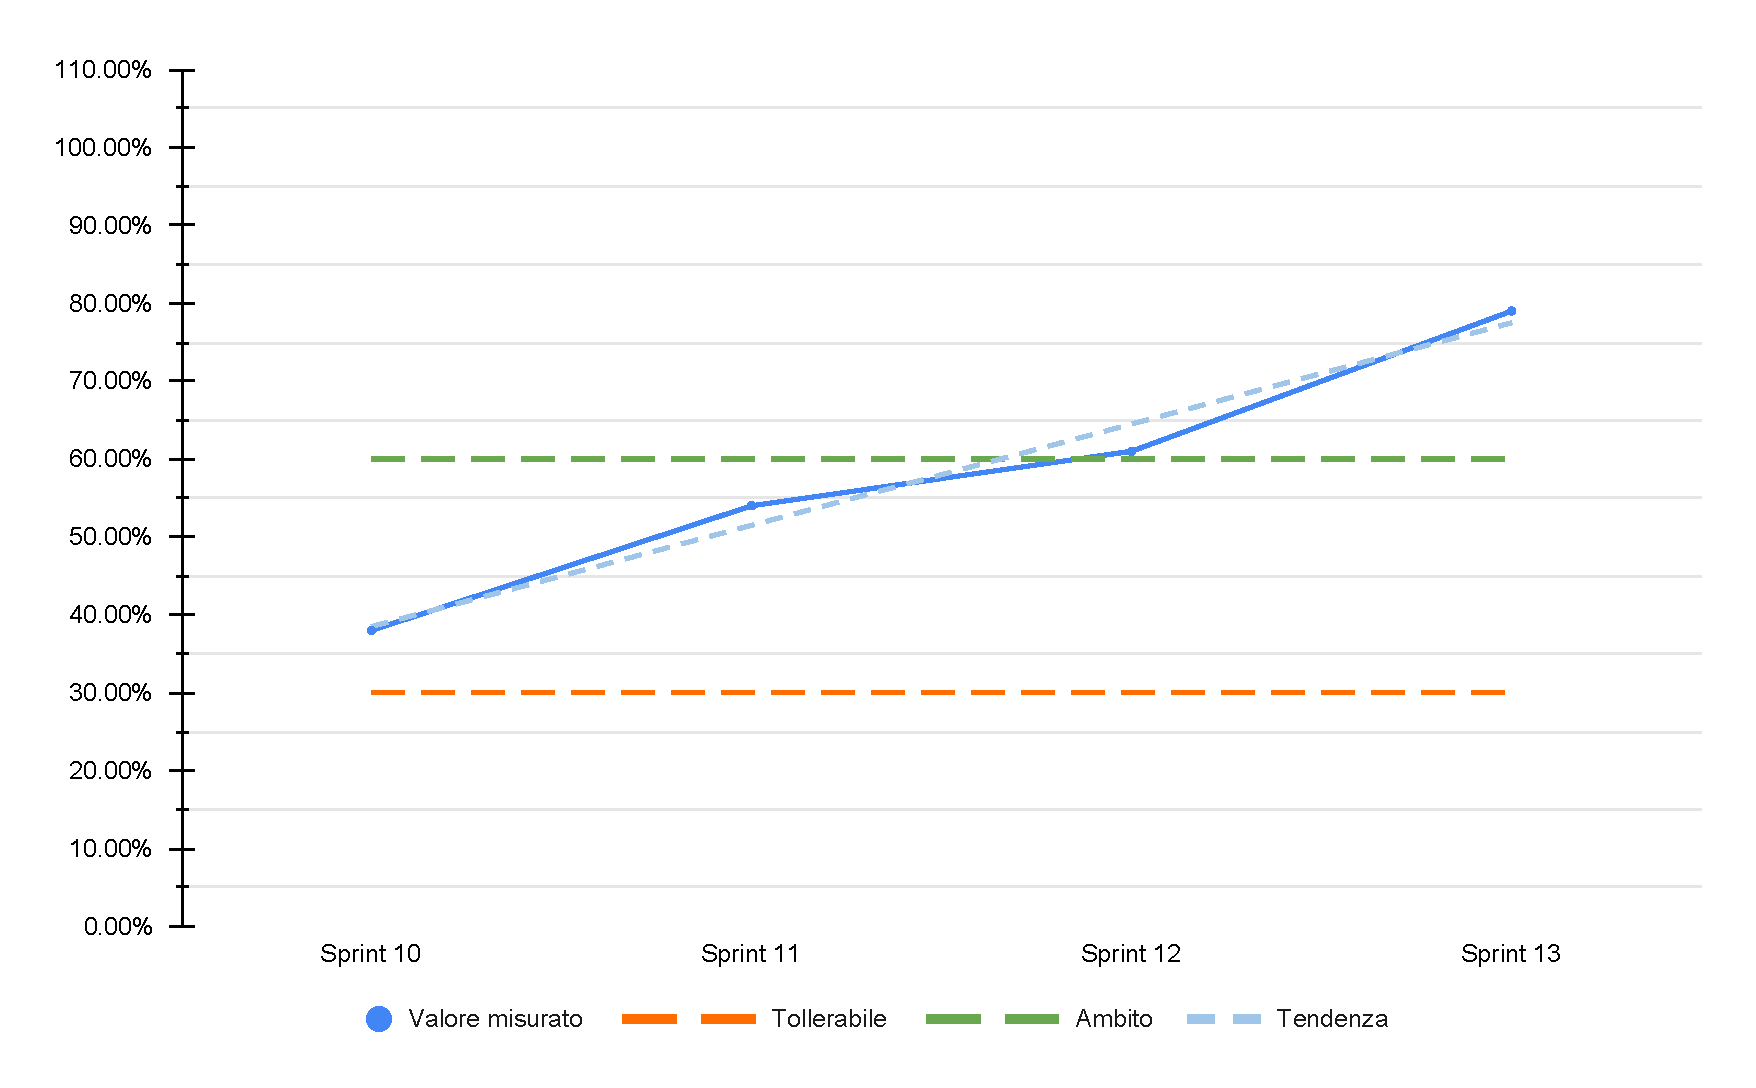
\includegraphics[width=\textwidth]{assets/requisiti_desiderabili_soddisfatti.pdf}
    \caption{M.PD.2 - Percentuale di requisiti desiderabili soddisfatti}
\end{figure}

\par Nell'arco della \glossario{PB}, la copertura dei requisiti desiderabili è rimasta costantemente entro i limiti di tollerabilità. Ciò è stato possibile grazie al fatto che alcuni di questi requisiti, come l'impiego di \glossario{Docker} e l'aggiunta di una funzionalità di \glossario{debug}, erano già stati soddisfatti durante la \glossario{RTB}. Questo ha permesso al team di migliorare progressivamente la percentuale di copertura, fino a superare il valore ambito. Oltre ad essere distribuita e sviluppata utilizzando Docker, l'applicazione è stata testata con Docker stesso. I requisiti non soddisfatti riguardano principalmente aspetti di accessibilità, come il contrasto dei colori e la visualizzazione di informazioni aggiuntive riguardanti i \glossario{dizionari dati}.